\documentclass[12pt,a4paper]{article}

\usepackage[spanish]{babel}
\usepackage{iftex}
\ifPDFTeX
    \usepackage[utf8]{inputenc}
    \usepackage[T1]{fontenc}
    \usepackage{newtxtext}
\else
    \usepackage{fontspec}
    \setmainfont{Times New Roman}
\fi
\usepackage{geometry}
\usepackage{graphicx}
\usepackage{booktabs}
\usepackage{array}
\usepackage{float}
\usepackage{amsmath}
\usepackage{caption}
\usepackage{longtable}
\usepackage{xcolor}
\usepackage{listings}
\usepackage{setspace}
\usepackage{hyperref}
\usepackage{algorithm}
\usepackage{algpseudocode}
\usepackage[most]{tcolorbox}

\geometry{margin=2.5cm}
\graphicspath{{graficos/}}
\setlength{\emergencystretch}{2em}
\renewcommand{\tablename}{Cuadro}
\floatname{algorithm}{Algoritmo}
\hypersetup{
    colorlinks=true,
    linkcolor=black,
    citecolor=black,
    urlcolor=blue
}

\lstdefinestyle{codigo}{
    basicstyle=\ttfamily\small,
    frame=tb,
    breaklines=true,
    backgroundcolor=\color{gray!5},
    columns=fullflexible,
    keepspaces=true,
    showstringspaces=false,
    numbers=left,
    numberstyle=\scriptsize\color{gray!70},
    numbersep=10pt,
    xleftmargin=2.2em,
    framexleftmargin=1.8em,
    captionpos=t
}

\newtcolorbox{cajaformula}{
    enhanced,
    colback=blue!3,
    colframe=blue!45!black,
    boxrule=0.8pt,
    arc=2mm,
    left=8mm,
    right=8mm,
    top=3mm,
    bottom=3mm,
    width=0.96\textwidth,
    center,
    drop shadow=black!12
}

\newcommand{\formula}[1]{
\begin{cajaformula}
\centering
#1
\end{cajaformula}
}

\begin{document}

\setstretch{1.28}
\setlength{\parskip}{0.35em}
\raggedbottom

\begin{center}
    \vspace*{0.8cm}
    {\Large\bfseries Análisis de Dependencia entre Variables Discretas\par}
    \vspace{0.25cm}
    {\Large\bfseries mediante Información Mutua y Árboles de Máxima\par}
    \vspace{0.25cm}
    {\Large\bfseries Expansión con Prim y Kruskal\par}

    \vspace{0.9cm}
    {\normalsize Apaza Anahui Waldir Alexander\par}

    \vspace{0.35cm}
    {\small Código fuente disponible en:
    \href{https://github.com/lexiwal19/Entropia.git}{\texttt{https://github.com/lexiwal19/Entropia.git}}\par}

    \vspace{0.25cm}
    {\small Video de exposición:
    \href{https://colocar-aqui-el-link-del-video}{\texttt{https://colocar-aqui-el-link-del-video}}\par}

    \vspace{0.45cm}
    {\normalsize 7 de julio de 2026\par}
\end{center}

\vspace{0.6cm}

\section*{Resumen}

El presente informe describe el procesamiento del dataset \texttt{d9\_strong.csv} mediante entropía de Shannon, información mutua y árboles de máxima dependencia. El flujo se implementó en Python de forma modular: el archivo \texttt{main.py} solo coordina las fases, mientras que los cálculos, gráficos, fórmulas y procesamiento del dataset fueron separados en archivos independientes.

El dataset original contiene 1000 registros y 9 variables: \(x1,x2,x5,x4,x6,x9,x3,x7,x8\). Las variables \(x7\) y \(x8\) fueron validadas y coincidieron en todos los registros. Por ello, se creó una variable objetivo \(Y\), donde \(Y=1\) representa la clase \textit{BEST} y \(Y=0\) representa la clase \textit{WORST}. La partición produjo 502 registros en \textit{BEST} y 498 registros en \textit{WORST}.

Luego se retiró \(Y\) de cada subconjunto, porque dentro de cada clase es constante y su entropía es cero. Con las variables restantes se calcularon entropías individuales, matrices de información mutua, grafos ponderados completos, árboles de máxima dependencia con Prim y Kruskal, y una comparación final basada en la suma de caminos de los árboles.

\textbf{Palabras clave:} entropía, información mutua, Shannon, Prim, Kruskal, árbol de máxima dependencia, dataset discreto.

\section{Introducción}

La entropía y la información mutua permiten estudiar relaciones entre variables discretas sin asumir una forma lineal. En este proyecto se analiza cómo se relacionan las variables de un dataset categórico y cómo cambia esa estructura al dividir los registros en dos clases: \textit{BEST} y \textit{WORST}.

El objetivo no es entrenar un modelo predictivo, sino resumir la dependencia entre variables mediante un grafo ponderado. Cada nodo representa una variable y cada arista usa como peso la información mutua entre dos variables. A partir de ese grafo se obtiene un árbol de máxima dependencia, que conserva las relaciones más importantes sin formar ciclos.

\section{Caracterización del conjunto de datos}

El archivo utilizado fue \texttt{d9\_strong.csv}. El conjunto contiene 1000 observaciones y 9 variables discretas/categóricas. No se detectaron valores faltantes durante el procesamiento. La Tabla \ref{tab:resumen_dataset} resume las características principales.

\begin{table}[H]
\centering
\caption{Resumen del conjunto de datos}
\label{tab:resumen_dataset}
\begin{tabular}{lc}
\toprule
\textbf{Característica} & \textbf{Valor} \\
\midrule
Registros & 1000 \\
Variables originales & 9 \\
Valores faltantes & 0 \\
Tipo de variables & Discretas/categóricas \\
Aristas del grafo completo original & 36 \\
Aristas esperadas en el árbol original & 8 \\
Registros BEST & 502 \\
Registros WORST & 498 \\
\bottomrule
\end{tabular}
\end{table}

\subsection{Dominio y cardinalidad}

Las variables se encuentran codificadas con valores enteros. La Tabla \ref{tab:dominios} muestra el dominio observado y la cantidad de categorías de cada variable.

\begin{table}[H]
\centering
\caption{Dominio y cardinalidad de las variables}
\label{tab:dominios}
\begin{tabular}{lcc}
\toprule
\textbf{Variable} & \textbf{Dominio} & \textbf{Categorías} \\
\midrule
\(x1\) & \(\{0,1\}\) & 2 \\
\(x2\) & \(\{0,1\}\) & 2 \\
\(x5\) & \(\{0,1,2\}\) & 3 \\
\(x4\) & \(\{0,1\}\) & 2 \\
\(x6\) & \(\{0,1\}\) & 2 \\
\(x9\) & \(\{0,1,2,3\}\) & 4 \\
\(x3\) & \(\{0,1,2\}\) & 3 \\
\(x7\) & \(\{0,1\}\) & 2 \\
\(x8\) & \(\{0,1\}\) & 2 \\
\bottomrule
\end{tabular}
\end{table}

\subsection{Verificación de calidad}

Se verificó que las variables \(x7\) y \(x8\) coinciden en los 1000 registros. Por ese motivo se creó la variable objetivo \(Y\), conservando la interpretación \(Y=1\) para \textit{BEST} y \(Y=0\) para \textit{WORST}. Luego, \(Y\) se retiró de cada subconjunto porque dentro de cada clase es constante.

\section{Objetivos}

\subsection{Objetivo general}

Analizar el dataset \texttt{d9\_strong.csv} mediante entropía de Shannon, información mutua y árboles de máxima dependencia, comparando los grupos \textit{BEST} y \textit{WORST}.

\subsection{Objetivos específicos}

\begin{itemize}
    \item Validar las variables \(x7\) y \(x8\) para construir la variable objetivo \(Y\).
    \item Dividir el dataset en dos grupos: \textit{BEST} y \textit{WORST}.
    \item Retirar \(Y\) de cada grupo para analizar solo las variables internas.
    \item Calcular la entropía individual de cada variable.
    \item Calcular matrices de información mutua para cada grupo.
    \item Construir grafos ponderados completos usando información mutua como peso.
    \item Obtener árboles de máxima dependencia mediante Prim y Kruskal.
    \item Comparar los resultados de \textit{BEST} y \textit{WORST}.
\end{itemize}

\section{Organización del proyecto}

El código fue dividido para evitar que el archivo principal quede saturado. La Tabla \ref{tab:organizacion} resume la estructura usada.

\begin{table}[H]
\centering
\caption{Organización modular del proyecto}
\label{tab:organizacion}
\begin{tabular}{p{5cm}p{9cm}}
\toprule
\textbf{Archivo o carpeta} & \textbf{Descripción} \\
\midrule
\texttt{main.py} & Archivo principal. Ejecuta el flujo fase por fase y pausa entre etapas. \\
\texttt{config.py} & Define rutas, columnas esperadas y carpetas de salida. \\
\texttt{utilidades.py} & Contiene funciones de impresión, pausa, guardado CSV y soporte visual. \\
\texttt{formulas.py} & Contiene entropía, información mutua, matriz IM, Prim, Kruskal y matriz de caminos. \\
\texttt{graficos.py} & Genera mapas de calor, grafos ponderados y árboles en formato PNG. \\
\texttt{fases\_dataset.py} & Carga el dataset, valida \(x7,x8\), crea \(Y\), divide y retira \(Y\). \\
\texttt{fases\_informacion.py} & Ejecuta entropía individual y matriz de información mutua. \\
\texttt{fases\_grafos.py} & Construye grafos, árboles y comparación final. \\
\texttt{salidas/datasets/} & Guarda datasets generados durante el proceso. \\
\texttt{salidas/tablas/} & Guarda matrices, aristas, árboles y comparaciones en CSV. \\
\texttt{graficos/} & Guarda todas las imágenes utilizadas en el informe. \\
\bottomrule
\end{tabular}
\end{table}

\section{Fundamento teórico}

\subsection{Entropía de Shannon}

La entropía mide la incertidumbre de una variable discreta \(X\). Si \(X\) toma valores \(x\) con probabilidad \(P(x)\), entonces:

\formula{
\[
H(X)=-\sum_x P(x)\log_2 P(x)
\]
}

Si todos los valores son muy predecibles, la entropía es baja. Si los valores están más distribuidos, la entropía aumenta.

\subsection{Información mutua}

La información mutua mide cuánta información comparte una variable con otra. Para dos variables discretas \(X\) y \(Y\):

\formula{
\[
I(X;Y)=\sum_x\sum_y P(x,y)\log_2\left(\frac{P(x,y)}{P(x)P(y)}\right)
\]
}

Si \(I(X;Y)=0\), las variables son independientes o casi independientes. Si el valor aumenta, la dependencia también aumenta.

\subsection{Grafo ponderado por información mutua}

Cada variable es un nodo y cada arista se pondera con información mutua:

\formula{
\[
w(x_i,x_j)=I(x_i;x_j)
\]
}

La diagonal de la matriz no se usa como arista, porque \(I(X;X)\) equivale a la entropía de la misma variable.

\subsection{Árbol de máxima dependencia}

Un árbol de expansión conecta todos los nodos sin ciclos. En este proyecto se busca el árbol que maximiza la suma de pesos:

\formula{
\[
W(T)=\sum_{(u,v)\in T} I(u;v)
\]
}

Se usa un árbol de máxima dependencia porque los pesos representan relación informativa. A mayor peso, mayor dependencia entre variables.

\section{Metodología}

El proceso se ejecutó por fases:

\begin{enumerate}
    \item Carga y revisión del dataset original.
    \item Validación de \(x7\) y \(x8\).
    \item Creación de la variable \(Y\).
    \item División del dataset en \textit{BEST} y \textit{WORST}.
    \item Retiro de \(Y\) para análisis interno.
    \item Cálculo de entropías.
    \item Cálculo de matrices de información mutua.
    \item Construcción de grafos ponderados.
    \item Obtención de árboles por Prim y Kruskal.
    \item Comparación de caminos entre \textit{BEST} y \textit{WORST}.
\end{enumerate}

\subsection{Construcción de la variable Y}

En el dataset se verificó que \(x7=x8\) en los 1000 registros. Por ello, se definió:

\formula{
\[
Y=x7=x8
\]
}

La interpretación usada fue:

\begin{itemize}
    \item \(Y=1\): clase \textit{BEST}.
    \item \(Y=0\): clase \textit{WORST}.
\end{itemize}

Para ordenar y dividir los valores de \(Y\) no se utilizo un algoritmo de aprendizaje automatico. Se aplico una regla deterministica de clasificacion por etiqueta binaria. Primero, el dataset se ordeno de forma descendente usando la columna \(Y\), de modo que los registros con \(Y=1\) quedaran antes que los registros con \(Y=0\). Luego, la separacion se hizo mediante filtrado booleano:

\formula{
\[
BEST=\{r \in D \mid Y(r)=1\}, \qquad WORST=\{r \in D \mid Y(r)=0\}
\]
}

En la implementacion de Python, este procedimiento corresponde a \texttt{sort\_values(by="Y", ascending=False)} para el ordenamiento y a condiciones del tipo \texttt{df[df["Y"] == 1]} y \texttt{df[df["Y"] == 0]} para la division.

\begin{table}[H]
\centering
\caption{Distribución final de registros}
\label{tab:distribucion}
\begin{tabular}{lcc}
\toprule
\textbf{Grupo} & \textbf{Condición} & \textbf{Registros} \\
\midrule
\textit{BEST} & \(Y=1\) & 502 \\
\textit{WORST} & \(Y=0\) & 498 \\
\textbf{Total} & -- & 1000 \\
\bottomrule
\end{tabular}
\end{table}

\section{Algoritmos}

\subsection{Cálculo de información mutua}

\begin{algorithm}[H]
\caption{Cálculo de información mutua entre dos variables discretas}
\begin{algorithmic}[1]
\Require Variables discretas \(X\), \(Y\)
\Ensure Valor \(I(X;Y)\)
\State \(IM \gets 0\)
\ForAll{\(x \in dominio(X)\)}
    \ForAll{\(y \in dominio(Y)\)}
        \State Calcular \(P(x)\), \(P(y)\), \(P(x,y)\)
        \If{\(P(x,y)>0\)}
            \State \(IM \gets IM + P(x,y)\log_2\left(\frac{P(x,y)}{P(x)P(y)}\right)\)
        \EndIf
    \EndFor
\EndFor
\State \Return \(IM\)
\end{algorithmic}
\end{algorithm}

\subsection{Kruskal para máxima dependencia}

\begin{algorithm}[H]
\caption{Kruskal para árbol de máxima dependencia}
\begin{algorithmic}[1]
\Require Grafo completo \(G=(V,E)\) con pesos \(I(X_i;X_j)\)
\Ensure Árbol de máxima dependencia \(T\)
\State Ordenar aristas de mayor a menor peso
\State \(T \gets \emptyset\)
\ForAll{arista \((u,v)\) en orden descendente}
    \If{\((u,v)\) no forma ciclo en \(T\)}
        \State Agregar \((u,v)\) a \(T\)
    \EndIf
    \If{\(|T|=|V|-1\)}
        \State detener
    \EndIf
\EndFor
\State \Return \(T\)
\end{algorithmic}
\end{algorithm}

\subsection{Prim para máxima dependencia}

\begin{algorithm}[H]
\caption{Prim para árbol de máxima dependencia}
\begin{algorithmic}[1]
\Require Grafo completo \(G=(V,E)\)
\Ensure Árbol de máxima dependencia \(T\)
\State Elegir un nodo inicial
\State \(T \gets \emptyset\)
\State \(Visitados \gets \{nodo\ inicial\}\)
\While{\(|Visitados|<|V|\)}
    \State Elegir la arista de mayor peso que conecte un nodo visitado con uno no visitado
    \State Agregar la arista a \(T\)
    \State Marcar el nuevo nodo como visitado
\EndWhile
\State \Return \(T\)
\end{algorithmic}
\end{algorithm}

\section{Resultados}

\subsection{Entropías individuales}

\begin{table}[H]
\centering
\caption{Entropía individual por grupo}
\label{tab:entropias}
\begin{tabular}{lcc}
\toprule
\textbf{Variable} & \textbf{BEST} & \textbf{WORST} \\
\midrule
\(x1\) & 0.758564 & 0.735374 \\
\(x2\) & 0.999072 & 0.998592 \\
\(x5\) & 1.411587 & 1.416200 \\
\(x4\) & 0.747456 & 0.686015 \\
\(x6\) & 0.997422 & 0.999814 \\
\(x9\) & 1.744762 & 1.685441 \\
\(x3\) & 0.674114 & 0.743092 \\
\bottomrule
\end{tabular}
\end{table}

En \textit{BEST}, la variable con mayor entropía es \(x9\), con 1.744762 bits. En \textit{WORST}, también destaca \(x9\), con 1.685441 bits. Esto indica que \(x9\) conserva alta variabilidad en ambos grupos.

\begin{figure}[H]
\centering
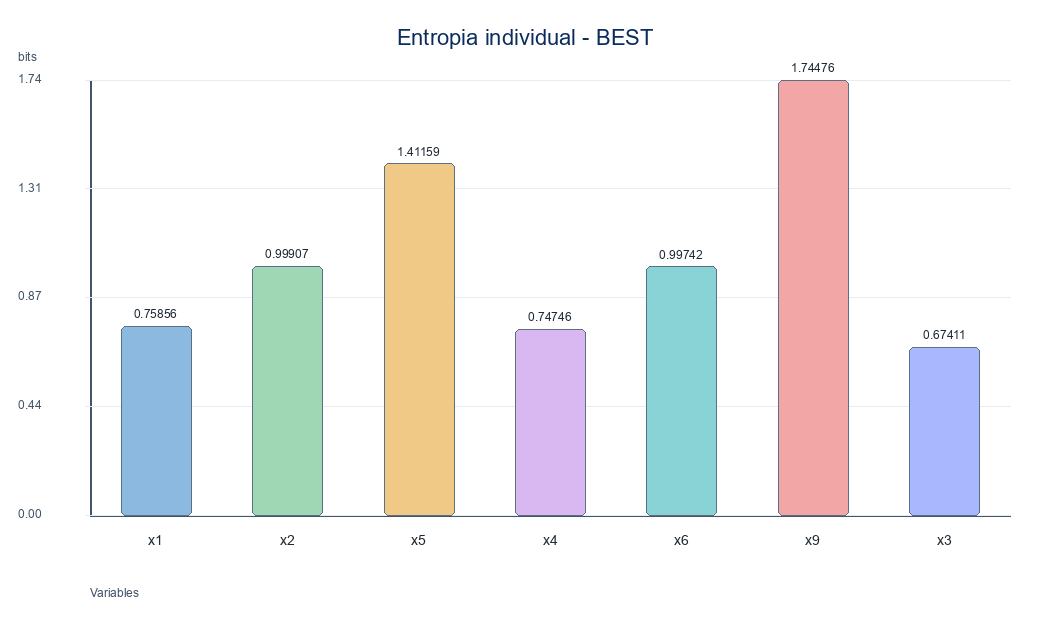
\includegraphics[width=\textwidth]{entropia_best.png}
\caption{Gráfico de barras de entropía individual para BEST}
\label{fig:entropia_best}
\end{figure}

\begin{figure}[H]
\centering
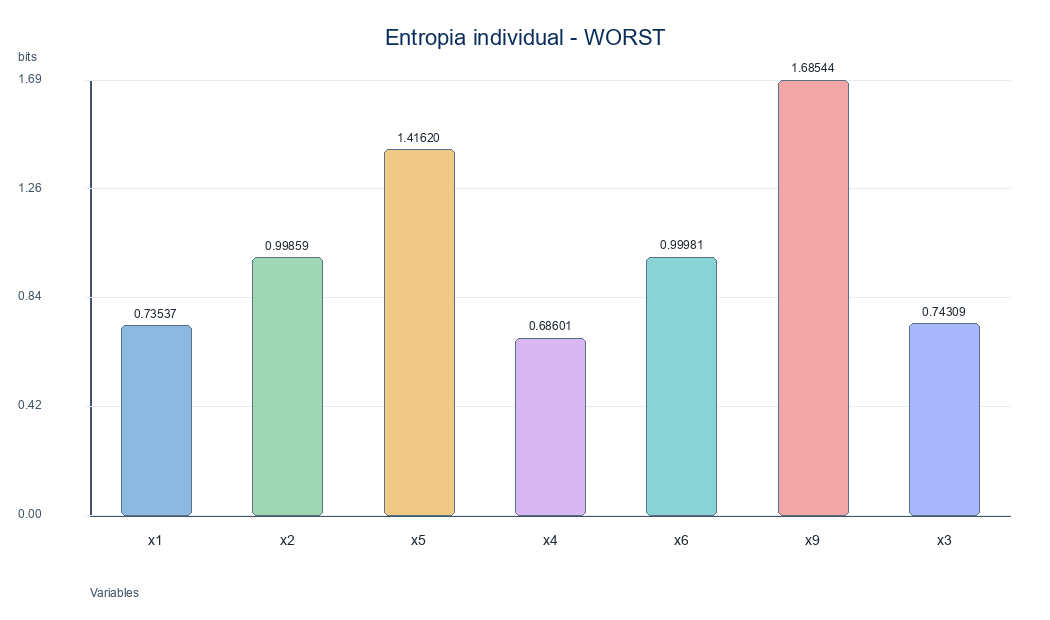
\includegraphics[width=\textwidth]{entropia_worst.png}
\caption{Gráfico de barras de entropía individual para WORST}
\label{fig:entropia_worst}
\end{figure}

\begin{figure}[H]
\centering
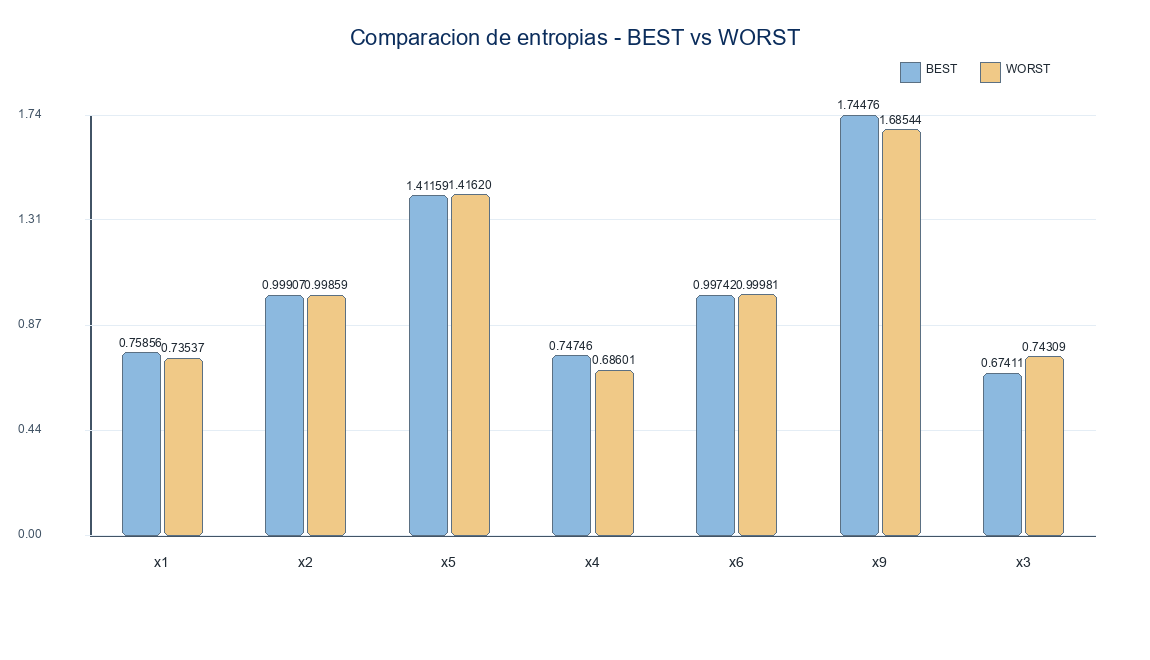
\includegraphics[width=\textwidth]{comparacion_entropias_best_worst.png}
\caption{Comparación de entropías por variable entre BEST y WORST}
\label{fig:comparacion_entropias}
\end{figure}

\subsection{Resultados del grupo BEST}

En el grupo \textit{BEST} se analizaron 502 registros. Las variables con mayor entropía fueron \(x9\), \(x5\), \(x2\) y \(x6\). En la matriz de información mutua se observa que las relaciones más fuertes son \(x6-x9\), \(x4-x9\), \(x2-x5\) y \(x1-x5\). Estas relaciones son las que finalmente dominan el árbol de máxima dependencia.

\subsection{Matriz de información mutua BEST}

\begin{table}[H]
\centering
\scriptsize
\caption{Matriz de información mutua para BEST}
\label{tab:im_best}
\begin{tabular}{lrrrrrrr}
\toprule
 & \(x1\) & \(x2\) & \(x5\) & \(x4\) & \(x6\) & \(x9\) & \(x3\) \\
\midrule
\(x1\) & 0.758564 & 0.002443 & 0.414958 & 0.000030 & 0.006396 & 0.006914 & 0.002232 \\
\(x2\) & 0.002443 & 0.999072 & 0.655467 & 0.001334 & 0.003924 & 0.005365 & 0.000753 \\
\(x5\) & 0.414958 & 0.655467 & 1.411587 & 0.006290 & 0.009532 & 0.016187 & 0.000722 \\
\(x4\) & 0.000030 & 0.001334 & 0.006290 & 0.747456 & 0.000116 & 0.747456 & 0.000000 \\
\(x6\) & 0.006396 & 0.003924 & 0.009532 & 0.000116 & 0.997422 & 0.997422 & 0.000106 \\
\(x9\) & 0.006914 & 0.005365 & 0.016187 & 0.747456 & 0.997422 & 1.744762 & 0.000107 \\
\(x3\) & 0.002232 & 0.000753 & 0.000722 & 0.000000 & 0.000106 & 0.000107 & 0.674114 \\
\bottomrule
\end{tabular}
\end{table}

\begin{figure}[H]
\centering
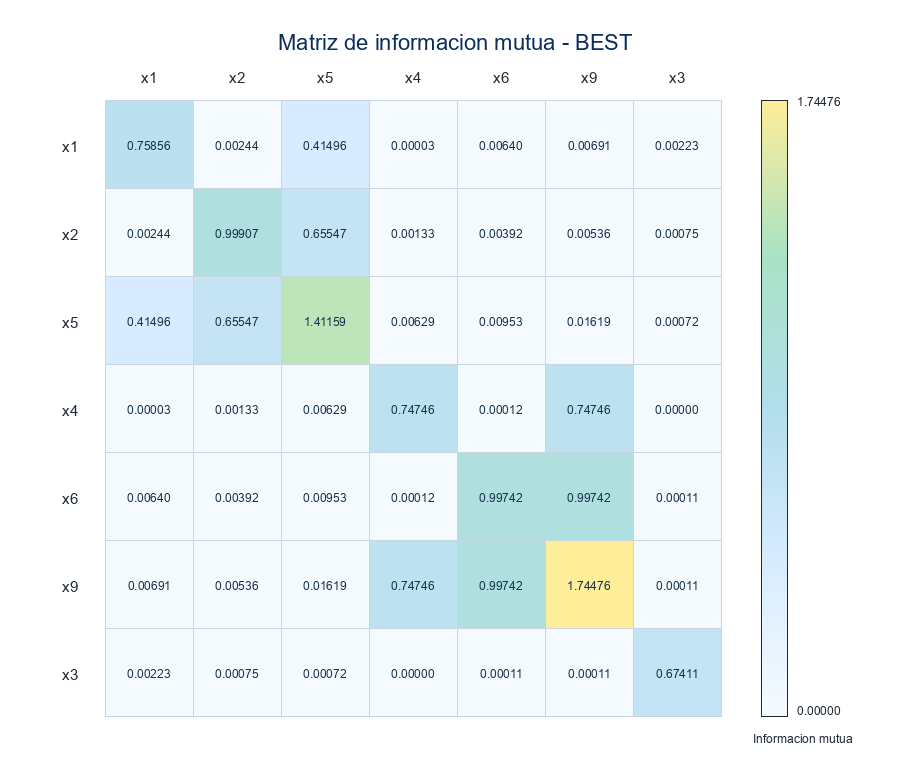
\includegraphics[width=\textwidth]{heatmap_IM_best.png}
\caption{Mapa de calor de información mutua para BEST}
\label{fig:heatmap_best}
\end{figure}

\subsection{Grafo ponderado completo BEST}

El grafo completo de \textit{BEST} usa como peso cada valor de información mutua entre pares de variables. Las relaciones más fuertes son \(x6-x9\), \(x4-x9\), \(x2-x5\) y \(x1-x5\).

\begin{figure}[H]
\centering
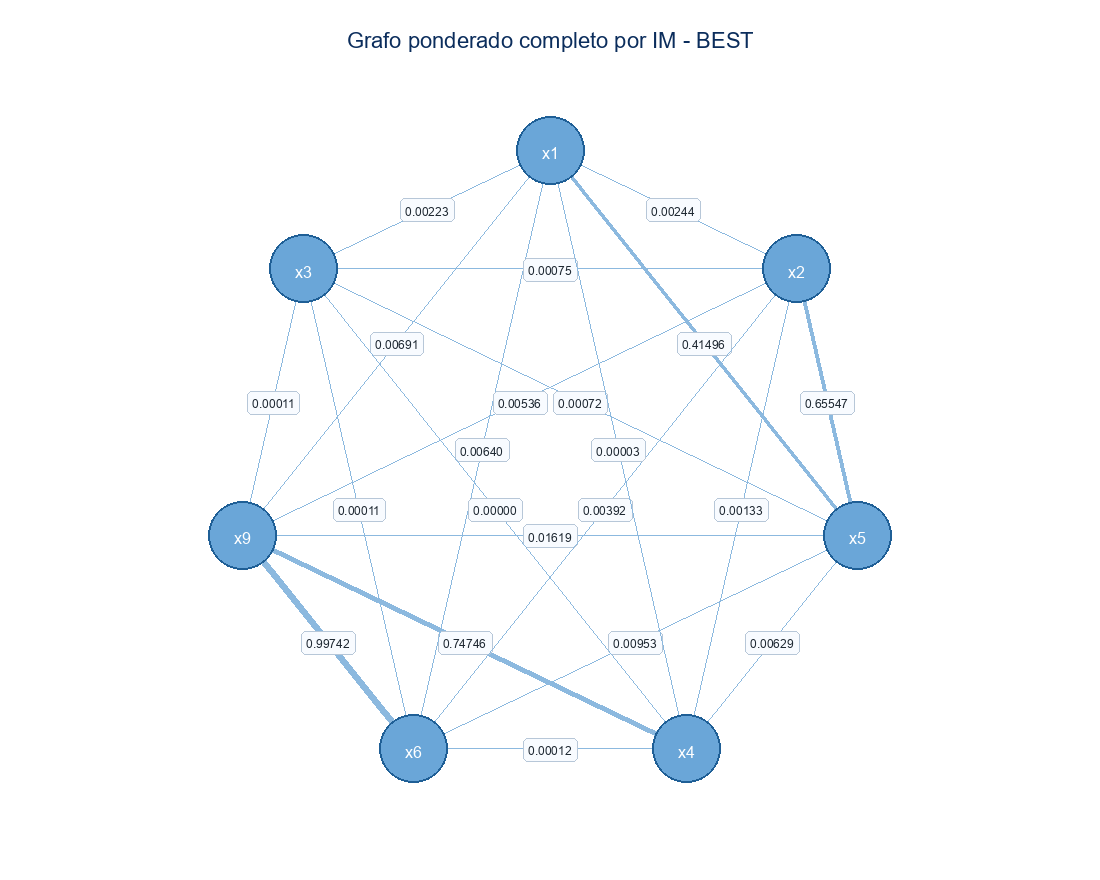
\includegraphics[width=\textwidth]{grafo_ponderado_best.png}
\caption{Grafo ponderado completo para BEST}
\label{fig:grafo_best}
\end{figure}

\subsection{Árbol de máxima dependencia BEST}

\begin{table}[H]
\centering
\caption{Árbol de máxima dependencia para BEST}
\label{tab:arbol_best}
\begin{tabular}{lc}
\toprule
\textbf{Arista} & \textbf{Peso IM} \\
\midrule
\(x6-x9\) & 0.997422 \\
\(x4-x9\) & 0.747456 \\
\(x2-x5\) & 0.655467 \\
\(x1-x5\) & 0.414958 \\
\(x5-x9\) & 0.016187 \\
\(x1-x3\) & 0.002232 \\
\bottomrule
\end{tabular}
\end{table}

El peso total del árbol \textit{BEST} es:

\formula{
\[
W(T_{BEST})=2.833722
\]
}

\begin{figure}[H]
\centering
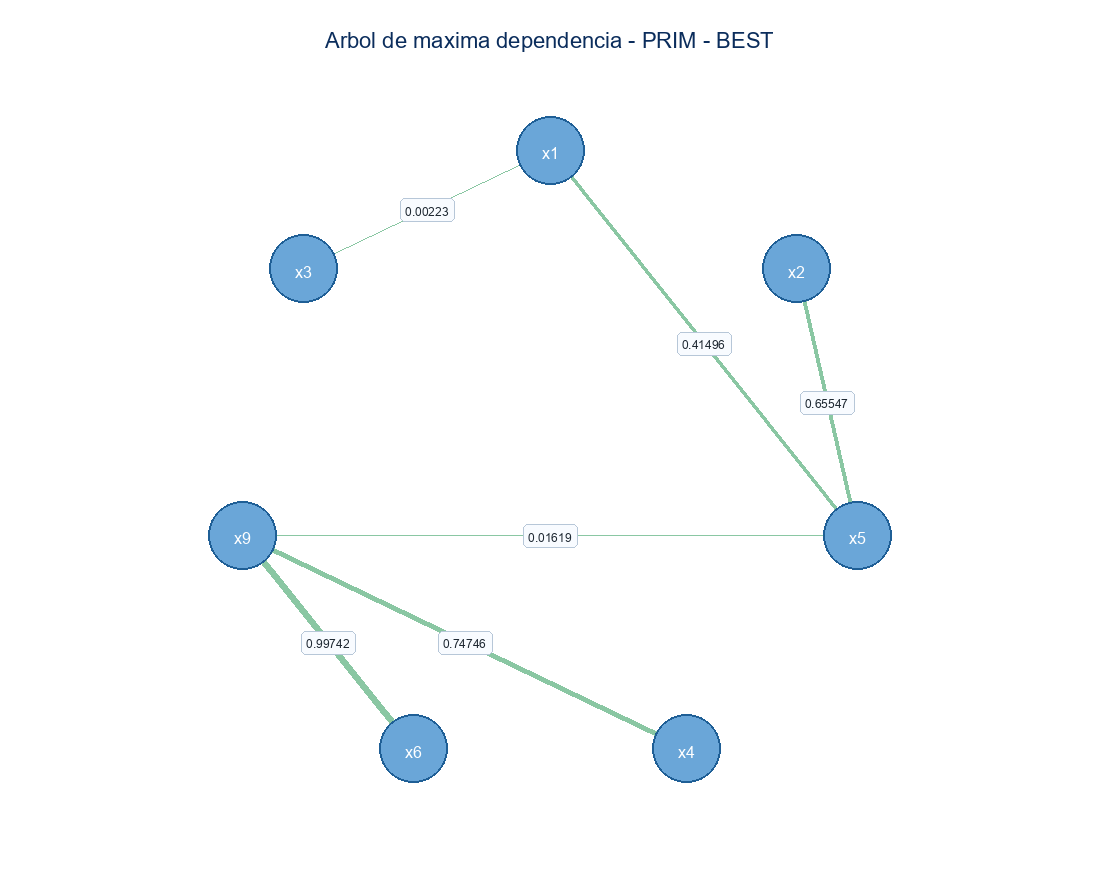
\includegraphics[width=\textwidth]{arbol_prim_best.png}
\caption{Árbol de máxima dependencia con Prim para BEST}
\label{fig:prim_best}
\end{figure}

\begin{figure}[H]
\centering
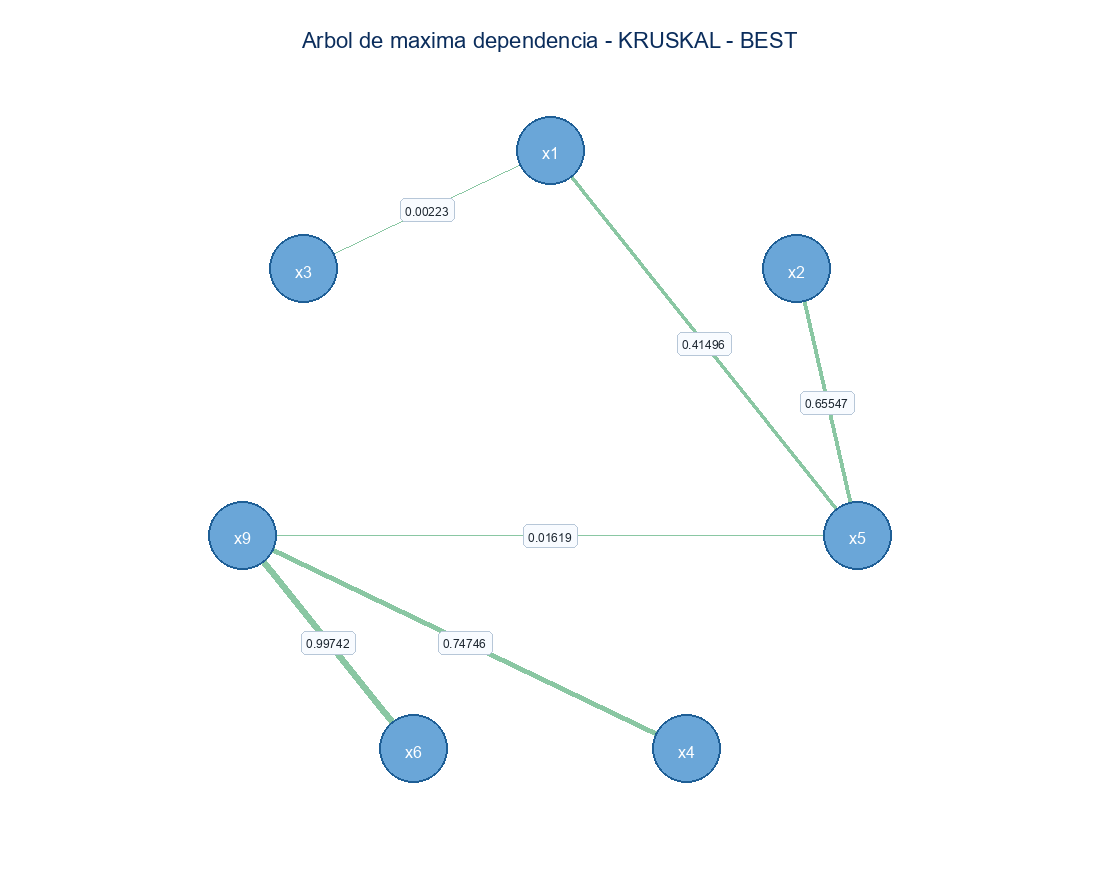
\includegraphics[width=\textwidth]{arbol_kruskal_best.png}
\caption{Árbol de máxima dependencia con Kruskal para BEST}
\label{fig:kruskal_best}
\end{figure}

\subsection{Resultados del grupo WORST}

En el grupo \textit{WORST} se analizaron 498 registros. Las variables con mayor entropía fueron \(x9\), \(x5\), \(x6\) y \(x2\). La estructura principal se mantiene parecida a BEST, aunque algunos pesos cambian. En particular, \(x2-x5\) aumenta en WORST, mientras que \(x4-x9\) disminuye respecto a BEST.

\subsection{Matriz de información mutua WORST}

\begin{table}[H]
\centering
\scriptsize
\caption{Matriz de información mutua para WORST}
\label{tab:im_worst}
\begin{tabular}{lrrrrrrr}
\toprule
 & \(x1\) & \(x2\) & \(x5\) & \(x4\) & \(x6\) & \(x9\) & \(x3\) \\
\midrule
\(x1\) & 0.735374 & 0.006098 & 0.423706 & 0.001810 & 0.000384 & 0.002923 & 0.000546 \\
\(x2\) & 0.006098 & 0.998592 & 0.686923 & 0.000020 & 0.000170 & 0.003140 & 0.000556 \\
\(x5\) & 0.423706 & 0.686923 & 1.416200 & 0.001194 & 0.000761 & 0.006917 & 0.001206 \\
\(x4\) & 0.001810 & 0.000020 & 0.001194 & 0.686015 & 0.000388 & 0.686015 & 0.004818 \\
\(x6\) & 0.000384 & 0.000170 & 0.000761 & 0.000388 & 0.999814 & 0.999814 & 0.000384 \\
\(x9\) & 0.002923 & 0.003140 & 0.006917 & 0.686015 & 0.999814 & 1.685441 & 0.005813 \\
\(x3\) & 0.000546 & 0.000556 & 0.001206 & 0.004818 & 0.000384 & 0.005813 & 0.743092 \\
\bottomrule
\end{tabular}
\end{table}

\begin{figure}[H]
\centering
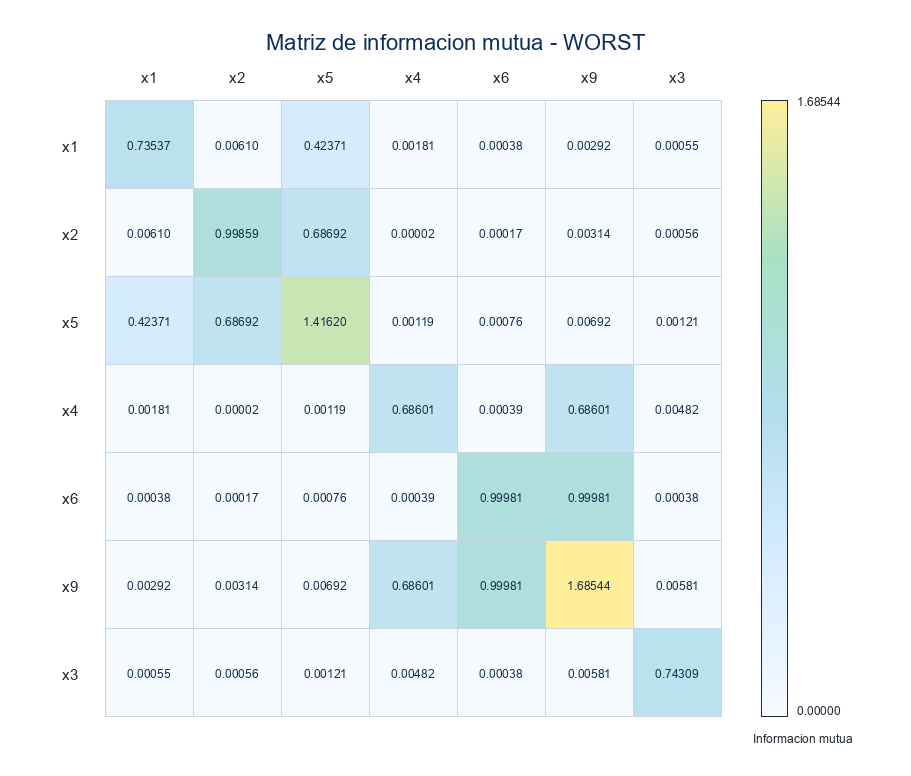
\includegraphics[width=\textwidth]{heatmap_IM_worst.png}
\caption{Mapa de calor de información mutua para WORST}
\label{fig:heatmap_worst}
\end{figure}

\begin{figure}[H]
\centering
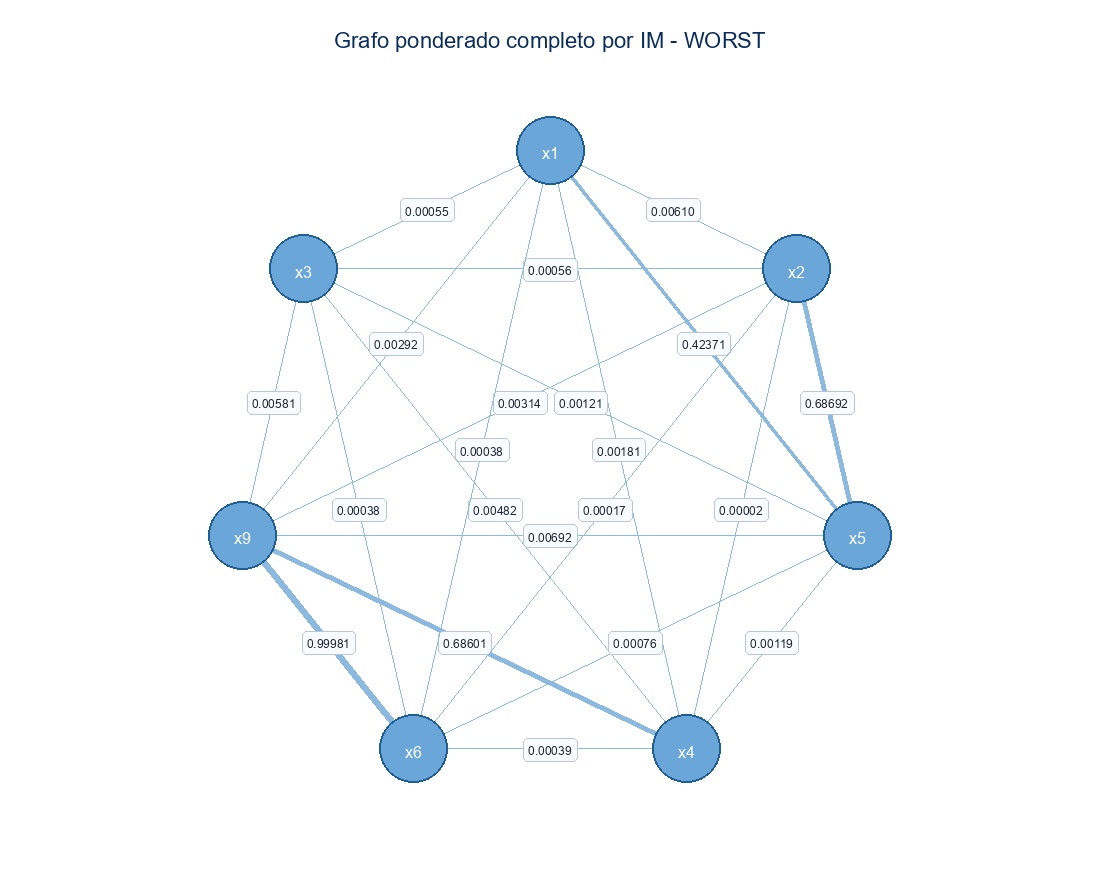
\includegraphics[width=\textwidth]{grafo_ponderado_worst.png}
\caption{Grafo ponderado completo para WORST}
\label{fig:grafo_worst}
\end{figure}

\begin{table}[H]
\centering
\caption{Árbol de máxima dependencia para WORST}
\label{tab:arbol_worst}
\begin{tabular}{lc}
\toprule
\textbf{Arista} & \textbf{Peso IM} \\
\midrule
\(x6-x9\) & 0.999814 \\
\(x2-x5\) & 0.686923 \\
\(x4-x9\) & 0.686015 \\
\(x1-x5\) & 0.423706 \\
\(x5-x9\) & 0.006917 \\
\(x9-x3\) & 0.005813 \\
\bottomrule
\end{tabular}
\end{table}

El peso total del árbol \textit{WORST} es:

\formula{
\[
W(T_{WORST})=2.809188
\]
}

\begin{figure}[H]
\centering
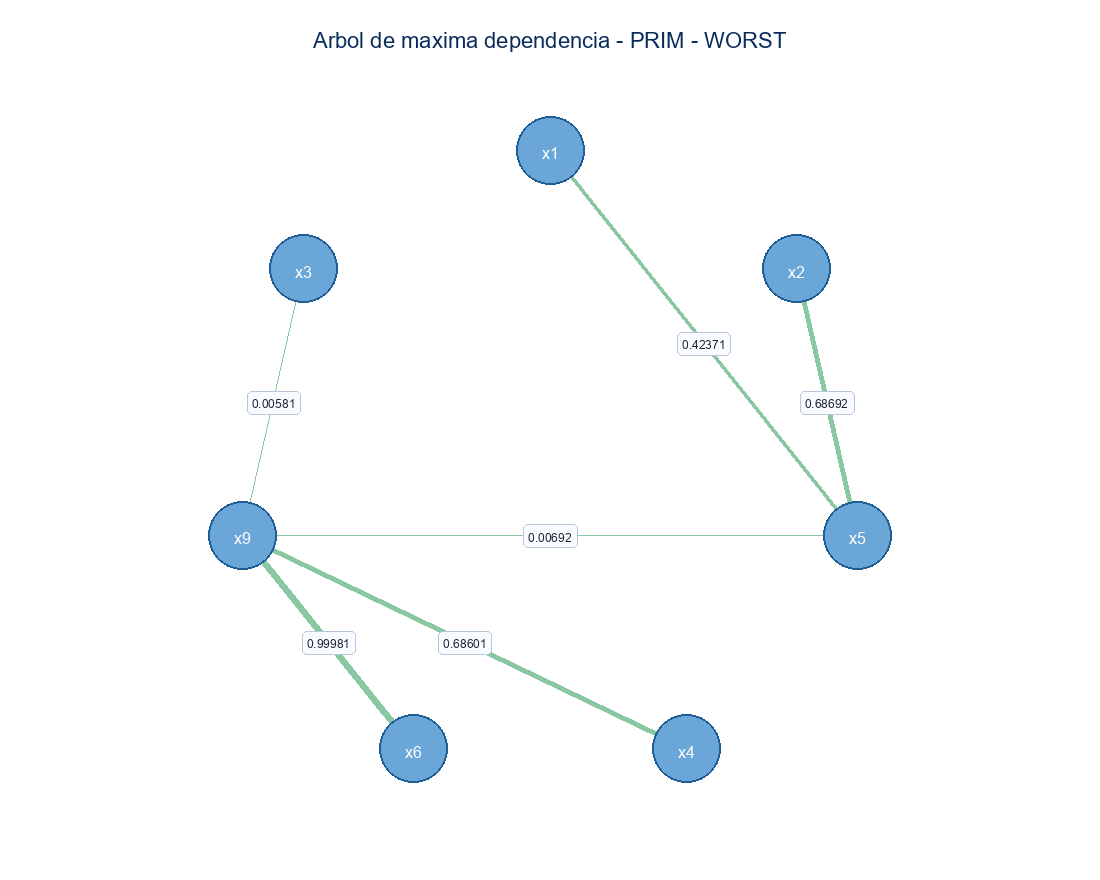
\includegraphics[width=\textwidth]{arbol_prim_worst.png}
\caption{Árbol de máxima dependencia con Prim para WORST}
\label{fig:prim_worst}
\end{figure}

\begin{figure}[H]
\centering
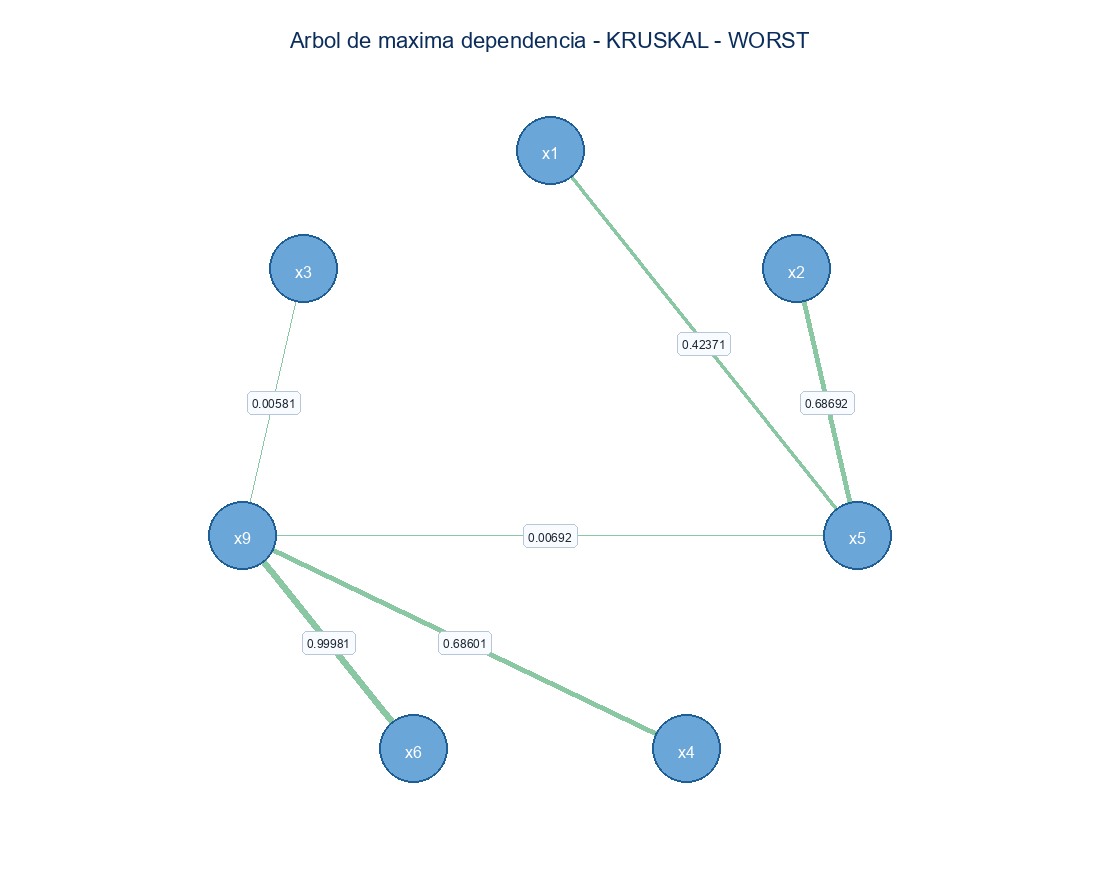
\includegraphics[width=\textwidth]{arbol_kruskal_worst.png}
\caption{Árbol de máxima dependencia con Kruskal para WORST}
\label{fig:kruskal_worst}
\end{figure}

\section{Comparación final}

\subsection{Matrices de suma de caminos}

La comparación final se realiza sobre el árbol de Kruskal. Para cada par de variables se calcula el único camino dentro del árbol y se suman los pesos de información mutua de sus aristas. Por ejemplo, si el camino entre \(x_i\) y \(x_j\) pasa por varias aristas, el valor almacenado es:

\formula{
\[
C(x_i,x_j)=\sum_{(u,v)\in camino(x_i,x_j)} I(u;v)
\]
}

\begin{table}[H]
\centering
\scriptsize
\caption{Matriz de suma de caminos para BEST}
\label{tab:matriz_caminos_best}
\begin{tabular}{lrrrrrrr}
\toprule
 & \(x1\) & \(x2\) & \(x3\) & \(x4\) & \(x5\) & \(x6\) & \(x9\) \\
\midrule
\(x1\) & 0.000000 & 1.070425 & 0.002232 & 1.178601 & 0.414958 & 1.428568 & 0.431145 \\
\(x2\) & 1.070425 & 0.000000 & 1.072657 & 1.419110 & 0.655467 & 1.669076 & 0.671654 \\
\(x3\) & 0.002232 & 1.072657 & 0.000000 & 1.180833 & 0.417190 & 1.430799 & 0.433377 \\
\(x4\) & 1.178601 & 1.419110 & 1.180833 & 0.000000 & 0.763643 & 1.744878 & 0.747456 \\
\(x5\) & 0.414958 & 0.655467 & 0.417190 & 0.763643 & 0.000000 & 1.013609 & 0.016187 \\
\(x6\) & 1.428568 & 1.669076 & 1.430799 & 1.744878 & 1.013609 & 0.000000 & 0.997422 \\
\(x9\) & 0.431145 & 0.671654 & 0.433377 & 0.747456 & 0.016187 & 0.997422 & 0.000000 \\
\bottomrule
\end{tabular}
\end{table}

\begin{table}[H]
\centering
\scriptsize
\caption{Matriz de suma de caminos para WORST}
\label{tab:matriz_caminos_worst}
\begin{tabular}{lrrrrrrr}
\toprule
 & \(x1\) & \(x2\) & \(x3\) & \(x4\) & \(x5\) & \(x6\) & \(x9\) \\
\midrule
\(x1\) & 0.000000 & 1.110629 & 0.436435 & 1.116638 & 0.423706 & 1.430436 & 0.430623 \\
\(x2\) & 1.110629 & 0.000000 & 0.699653 & 1.379855 & 0.686923 & 1.693654 & 0.693840 \\
\(x3\) & 0.436435 & 0.699653 & 0.000000 & 0.691828 & 0.012729 & 1.005627 & 0.005813 \\
\(x4\) & 1.116638 & 1.379855 & 0.691828 & 0.000000 & 0.692932 & 1.685829 & 0.686015 \\
\(x5\) & 0.423706 & 0.686923 & 0.012729 & 0.692932 & 0.000000 & 1.006730 & 0.006917 \\
\(x6\) & 1.430436 & 1.693654 & 1.005627 & 1.685829 & 1.006730 & 0.000000 & 0.999814 \\
\(x9\) & 0.430623 & 0.693840 & 0.005813 & 0.686015 & 0.006917 & 0.999814 & 0.000000 \\
\bottomrule
\end{tabular}
\end{table}

\subsection{Comparación por suma de caminos}

La comparación final se hizo usando el árbol de Kruskal. Para cada variable se sumaron los pesos acumulados de sus caminos hacia las demás variables. El resultado se muestra en la Tabla \ref{tab:comparacion_caminos}.

\begin{table}[H]
\centering
\caption{Comparación de recorridos acumulados}
\label{tab:comparacion_caminos}
\begin{tabular}{lrrrr}
\toprule
\textbf{Variable} & \textbf{Suma BEST} & \textbf{Suma WORST} & \textbf{Diferencia} & \textbf{Dif. abs.} \\
\midrule
\(x3\) & 4.537088 & 2.852084 & 1.685004 & 1.685004 \\
\(x4\) & 7.034521 & 6.253096 & 0.781426 & 0.781426 \\
\(x9\) & 3.297242 & 2.823021 & 0.474221 & 0.474221 \\
\(x6\) & 8.284353 & 7.822090 & 0.462263 & 0.462263 \\
\(x5\) & 3.281054 & 2.829937 & 0.451117 & 0.451117 \\
\(x1\) & 4.525929 & 4.948468 & -0.422538 & 0.422538 \\
\(x2\) & 6.558388 & 6.264555 & 0.293833 & 0.293833 \\
\bottomrule
\end{tabular}
\end{table}

La mayor diferencia se observa en \(x3\), con 1.685004. Esto ocurre porque \(x3\) se conecta al árbol por rutas distintas: en \textit{BEST} aparece la arista \(x1-x3\), mientras que en \textit{WORST} aparece \(x9-x3\).

\begin{figure}[H]
\centering
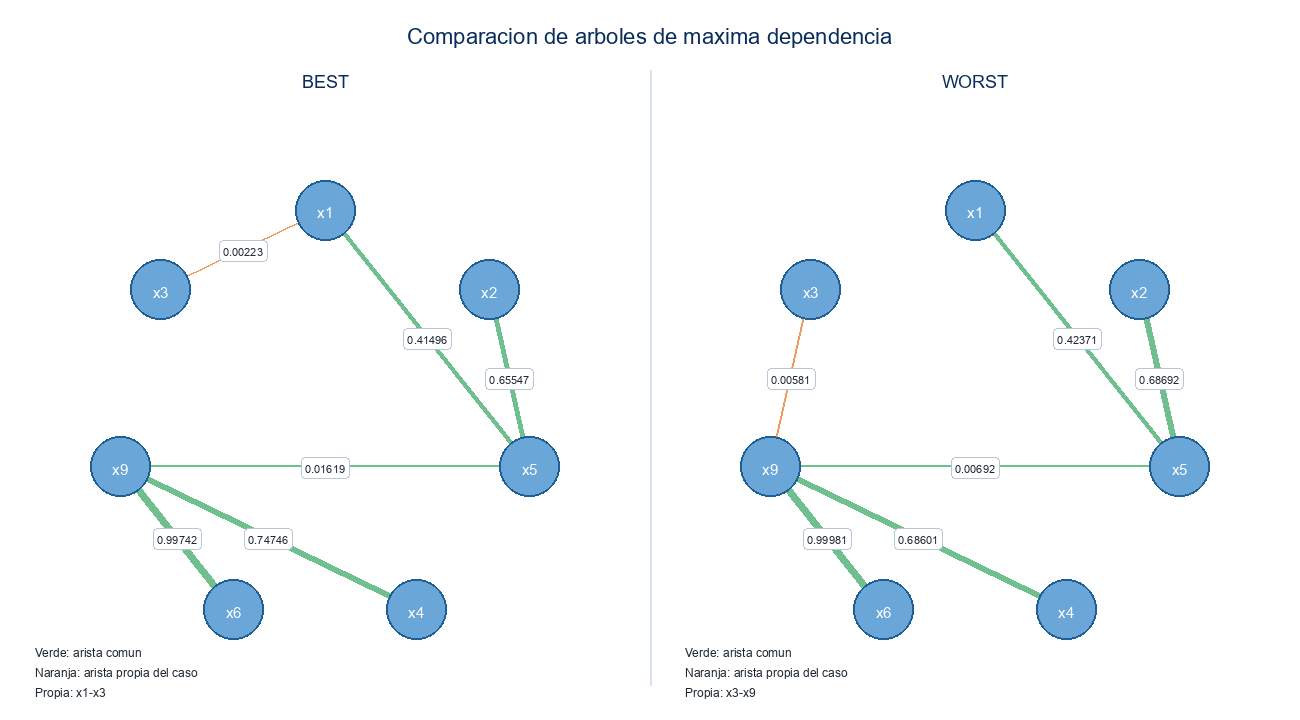
\includegraphics[width=\textwidth]{comparacion_arboles_best_worst.png}
\caption{Comparación visual de los árboles de máxima dependencia BEST y WORST}
\label{fig:comparacion_arboles}
\end{figure}

\subsection{Interpretación de los resultados}

\begin{itemize}
    \item En ambos grupos, \(x6-x9\) es la relación más fuerte.
    \item La relación \(x2-x5\) es más fuerte en \textit{WORST} que en \textit{BEST}.
    \item La relación \(x4-x9\) es más fuerte en \textit{BEST}.
    \item \(x3\) cambia su forma de conectarse al árbol según el grupo.
    \item Prim y Kruskal generan el mismo peso total dentro de cada grupo.
\end{itemize}

\section{Discusión}

La comparación muestra que \textit{BEST} y \textit{WORST} conservan una estructura central muy parecida. Las aristas \(x6-x9\), \(x4-x9\), \(x2-x5\), \(x1-x5\) y \(x5-x9\) aparecen como conexiones importantes dentro de los árboles. Esto indica que la partición por \(Y\) no destruye la estructura principal de dependencia.

La diferencia más clara está en \(x3\). En \textit{BEST}, \(x3\) se incorpora al árbol por medio de \(x1-x3\). En \textit{WORST}, \(x3\) se incorpora mediante \(x9-x3\). Aunque estos pesos son pequeños frente a relaciones como \(x6-x9\), son relevantes porque cambian la forma final del árbol.

En las entropías, \(x9\) mantiene el valor más alto en ambos casos. Esto significa que es una variable con mayor diversidad de valores y también aparece como nodo importante en los grafos. Por tanto, \(x9\) cumple un papel central tanto por variabilidad individual como por dependencia con otras variables.

Finalmente, Prim y Kruskal entregan el mismo peso total en cada grupo. Esto refuerza que los árboles obtenidos son consistentes con los pesos calculados y que la diferencia entre \textit{BEST} y \textit{WORST} se debe a los datos de cada clase, no al algoritmo usado.

\section{Conclusiones}

\begin{enumerate}
    \item El dataset contiene 1000 registros y las variables \(x7\) y \(x8\) coinciden en todos los casos, por lo que fue correcto construir \(Y=x7=x8\).
    \item La partición resultó balanceada: 502 registros en \textit{BEST} y 498 en \textit{WORST}.
    \item Al retirar \(Y\), se analizaron siete variables internas: \(x1,x2,x5,x4,x6,x9,x3\).
    \item La variable con mayor entropía en ambos grupos fue \(x9\), lo que indica mayor variabilidad.
    \item La relación más fuerte en ambos grupos fue \(x6-x9\).
    \item Los árboles de Prim y Kruskal coincidieron en peso total dentro de cada grupo.
    \item El árbol \textit{BEST} tuvo peso total 2.833722 y el árbol \textit{WORST} tuvo peso total 2.809188.
    \item La diferencia más importante aparece en \(x3\), porque cambia su conexión principal entre los dos grupos.
\end{enumerate}

\section*{Referencias}
\addcontentsline{toc}{section}{Referencias}

\begingroup
\setlength{\parindent}{0pt}
\setlength{\parskip}{1em}

Cover, T. M., \& Thomas, J. A. (2006). \textit{Elements of information theory}. Wiley.\par

Kruskal, J. B. (1956). On the shortest spanning subtree of a graph and the traveling salesman problem. \textit{Proceedings of the American Mathematical Society, 7}(1), 48--50.\par

Prim, R. C. (1957). Shortest connection networks and some generalizations. \textit{Bell System Technical Journal, 36}(6), 1389--1401.\par

Shannon, C. E. (1948). A mathematical theory of communication. \textit{Bell System Technical Journal, 27}(3), 379--423.\par

\endgroup

\end{document}
